\subsection{Напряженность электростатического поля. Поток напряженности ЭС поля. Теорема Гаусса в интегральной форме}

\begin{definition}
    Пусть $E_i$ - напряжённость электрического поля, создаваемая зарядом $q_i$ в точке с радиус-вектором
    $r_i$, проведенным из этого заряда. Тогда, из принципа суперпозиции электрических полей:

    $$
    \vec E=\sum_{i=1}^n\vec E_i=\frac{1}{4\pi\varepsilon_0}\sum_{i=1}^{n}\frac{q_i}{r^3_i}\vec r_i$$
\end{definition}

\begin{enumerate}
    \item Напряжённость электрического поля пространственно распределённого заряда
    
    $$\vec E=\int d\vec E=\frac{1}{4\pi\varepsilon_0}\int_V\frac{dq}{r^3}\vec r=\frac{1}{4\pi\varepsilon_0}\int_V\frac{\rho dV}{r^3}\vec r$$

    \item Напряжённость электрического поля распределённого по поверхности или линии заряда
    
    $$\vec E=\frac{1}{4\pi\varepsilon_0}\int_S\frac{dq}{r^3}\vec r=\frac{1}{4\pi\varepsilon_0}\int_S\frac{\sigma dS}{r^3}\vec r$$
    
    $$\vec E=\frac{1}{4\pi\varepsilon_0}\int_L\frac{dq}{r^3}\vec r=\frac{1}{4\pi\varepsilon_0}\int_L\frac{\lambda dl}{r^3}\vec r$$

\end{enumerate}

\begin{definition}
    Поток напряжённости ЭС поля.

    Скалярная величина:
    $$Ф_E=\int_SE\cos\alpha\ dS=\int_SE_п\ dS$$
\end{definition}

\begin{figure}[h]
    \centering
    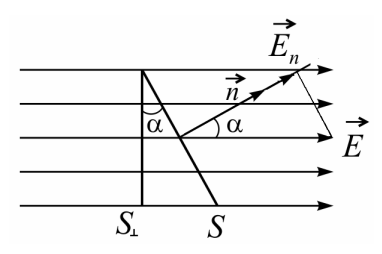
\includegraphics[width=0.5\linewidth]{imgs/q16i1.png}
\end{figure}

Рассмотрим площадку $S_\perp$, через которую проходит $N$ силовых линий:

$$E=\frac{N}{S_\perp}$$

Очевидно, столько же силовых линий проходит и через площадку $S$, расположенную под произвольным углом $\alpha$ к направлению силовых линий. $S_\perp=S\cos\alpha$

$$E=\frac{N}{S\cos\alpha}$$

$E\cos\alpha=E_п$ — проекция вектора $\vec E$ на направление нормали $\vec n$ к площадке $S$. 
В таком случае число силовых линий, пронизывающих произвольную площадку, размещенную в электрическом поле равно

$$N=ES\cos\alpha=E_пS$$

Если поле неоднородное, всегда можно выбрать элементарную площадку $dS$, 
которую можно считать плоской, а поле в ее окрестностях — однородным:

$$N=\int_SE_пdS$$

Правую часть уравнения выше называют потоком вектора $\vec E$ через поверхность $S$:

$$Ф_E=\int_SE\cos\alpha\ dS=\int_SE_п\ dS$$

или как скалярное произведение двух векторов, если поверхность замкнутая (за положительное направление нормали берем её внешнюю нормаль):

$$Ф_A^\circ=\int_S(\vec E\cdot\vec n)dS$$

Теорема Гаусса.

Поток вектора напряжённости электрического поля в вакууме через любую замкнутую поверхность равен 
алгебраической сумме зарядов, охваченных этой поверхностью, делённой на $\varepsilon_0$:

$$Ф_A^\circ=\sum_i\frac{q_i}{\varepsilon_0}$$

Интегральная форма:

$$Ф_E=\oint_S\vec Ed\vec S=\frac{1}{\varepsilon_0}\oint_V\rho\ dV$$

\begin{enumerate}
    \item Теорема Гаусса устанавливает фундаментальное свойство ЭП — наличие у него 
    источников (положительные заряды) и стоков (отрицательные заряды) линий поля.
    \item Теорема Гаусса позволяет вычислять напряженность поля систем дискретно и непрерывно распределенных зарядов, 
    т.е. выступает аналогом закона Кулона и принципа суперпозиции.
\end{enumerate}

Если заряд неравномерно распределён по объему.

$$\oint_S(\vec E, d\vec S)=\frac{\sum_iq_i}{\varepsilon_0}$$

Если электрические заряды распределены в разных местах пространства с некоторой объемной плотностью $\rho=\frac{dq}{dV}$, 
тогда суммарный заряд объема $dV$ будет равен $\sum q_i = \int p dV$.

Тогда:

$$Ф_E=\oint_S\vec Ed\vec S=\frac{1}{\varepsilon_0}\oint_V\rho\ dV$$
